\chapter{Background}
\label{chapter:background}

In this chapter, an introduction to deep learning the various 3D
geometry representations.  We begin by giving an introduction to
deep learning, including gradient descent and Convolutional Neural
Networks (CNN). This is followed by some details about 3D volumes and
their associated algorithms for voxelisation and surface extraction.


\section{Deep Learning}
\label{sec:background:nn}


\subsection{Gradient Descent}

Neural networks have significantly grown in size since their
inception. A neural network model of today may contain as many as
fifty million parameters. This establishes a difficult, extremely
large, non-convex optimisation problem. The only way to sensibly train
these models, ignoring minor implementation details, is to use
gradient descent optimisation.


To assist in the explanation of gradient descent, suppose a
classification problem with annotated training data
$Z = \{(x_i, y_i)\}$, containing images $x_i$ each with a
corresponding label $y_i$. We define $f$ as the classifier, mapping
image $x_i$ to label $y_i$ given a real vector of parameters $\theta$,
\begin{equation}
  y_i \approx f(x_i;\theta) .
\end{equation}

\noindent To measure the performance this classifier, a loss function
$\ell$ is defined, which is entirely dependant on the problem at
hand. Hence, our loss over $x$ is defined as,

\begin{equation}
  loss = \sum_i \ell(y_i, f(x_i ; \theta) .
\end{equation}


\noindent Initially parameters $\theta$ will be unknown. Hence, in
order to find $\theta$ (so that we can establish a trained
classifier), we must minimise the loss function,
\begin{equation}
  \min_\theta \sum_i \ell(y_i, f(x_i ; \theta)) .
\end{equation}



\noindent This minimisation is typically performed using gradient
descent, where $\theta$ is gradually learnt over many iterations. This
is at rate $\eta$ (known as the \textit{learning rate}), and is
directed by the gradient of the $f$ with parameters $\theta$,

\begin{equation}
  \theta = \theta - \eta \nabla_\theta \ell(y_i, f(x_i ; \theta) .
\end{equation}

More often than not, the above is extended to support batches of
images per iteration, which results in a more stable gradient due to
the averaging across several images.

\subsection{Convolutional Neural Networks}

In the previous subsection, an overview of gradient descent was
presented, where parameters $\theta$ were used to \textit{in some way}
to apply a mapping from image to label. Such a function might be
defined as simply as a linear function, $f(x;\theta) = \theta
x$. Unfortunately, despite being appropriate in many areas, a linear
function will struggle to map a non-linear problem, with is often the
case with computer vision based applications. As such, convolutions
are often used to both reduce the number of parameters, and to allow
convenient and efficient stacking, allowing the network learn
difficult mappings.

Convolutional Neural Networks (CNNs) are constructed, typically, from
stacks of convolutional filters, each followed by some form of
transfer function. The tailing end of a CNN is often specific to each
application. For example, for a numerical regression task, linear
layers may be added, and for segmentation, a $1\times 1$ convolution
may be added. As these networks have gradually increased in size, the
term \textit{Deep Learning} has become popular. Networks of today may
consist of several hundred convolutional layers, such as
ResNet-152~\cite{he2015deep}.

\subsection{Batch Normalisation}

As networks grew from 15 or so layers upwards, the job of gradient
descent became very difficult. During training, the distribution of
every input to every layer changes slightly. This is because the
parameters of the layer before each layer change. This problem is
referred to as \textit{internal covariate shift}. A solution known as
Batch Normalisation was proposed in~\cite{ioffe2015batch}, enabling
networks with many layers (such as the 152 layers in
ResNet~\cite{he2015deep}) to be trained in much shorter times. Some
additional advantages of using batch normalisation include being able
to use larger learning rates and reducing the need for such careful
initialisation.

Batch normalisation works as the name might suggest, by normalising
the output of each parameterised layer using learnable scale and shift
parameters, as well as the size of each minibatch, for each
minibatch. Understanding exactly how batch normalisation works is not
imperative to understanding the contents of this thesis. However, in
general, batch normalisation has been applied either before or after
every parameterised layer of the CNN models proposed in this
thesis. Additionally, as these networks are very large, they are
unlikely to have been possible to train without employing batch
normalisation.


\subsection{Frameworks}

While designing and developing a framework to work with deep neural
networks \textit{might} be an interesting thought experiment for some,
it is far from the focus of this thesis. The work presented throughout
this thesis was developed primarily under the
Torch~\footnote{\url{http://torch.ch/}, except for the work on facial
  part segmentation, which was developed under
  Cafe~\cite{jia2014caffe}}. There are a number of reasons for this,
but to name just a few:

\begin{enumerate}
\item Efficient GPU support. This is important, of course, in any
  framework intended for deep learning. Torch enables networks to be
  run in parallel (for speed) or sequentially (for additional memory)
  across multiple GPUs.
\item Elegant memory backend. Data can be loaded directly into memory
  and views can be applied to create $N$-dimensional Tensors without
  shuffling memory. This is very important when reading in large
  volumetric training samples.
\item Multithreading. The trade offs between I/O and CPU are discussed
  in more detail in Section~\ref{sec:background:volstorage}. However,
  regardless of how the data is optimised (in terms of compression or
  just raw data), volumes are big. Loading them sequentially and
  applying augmentation, even on very fast hardware, remains a
  computationally expensive task.
\end{enumerate}


\section{3D Volumes and Volumetric Algorithms}
\label{sec:background:volumes}

Typically, 3D models are provided as a mesh, defined by vertices and
faces, in a particular file format such as \textit{Wavefront
  Obj}. These files typically contain additional data, such as texture
mapping coordinates and surface normals. To represent the structure of
an object, only the mesh is required. However, an alternative approach
to representing the structure of an object is to encode it in a three
dimensional volume. This may be thought of as a 3D matrix, where
\textit{inside} the object is denoted by a one, and \textit{outside}
is denoted with a zero.

\begin{figure}
  \begin{tabular}{ccccc}
    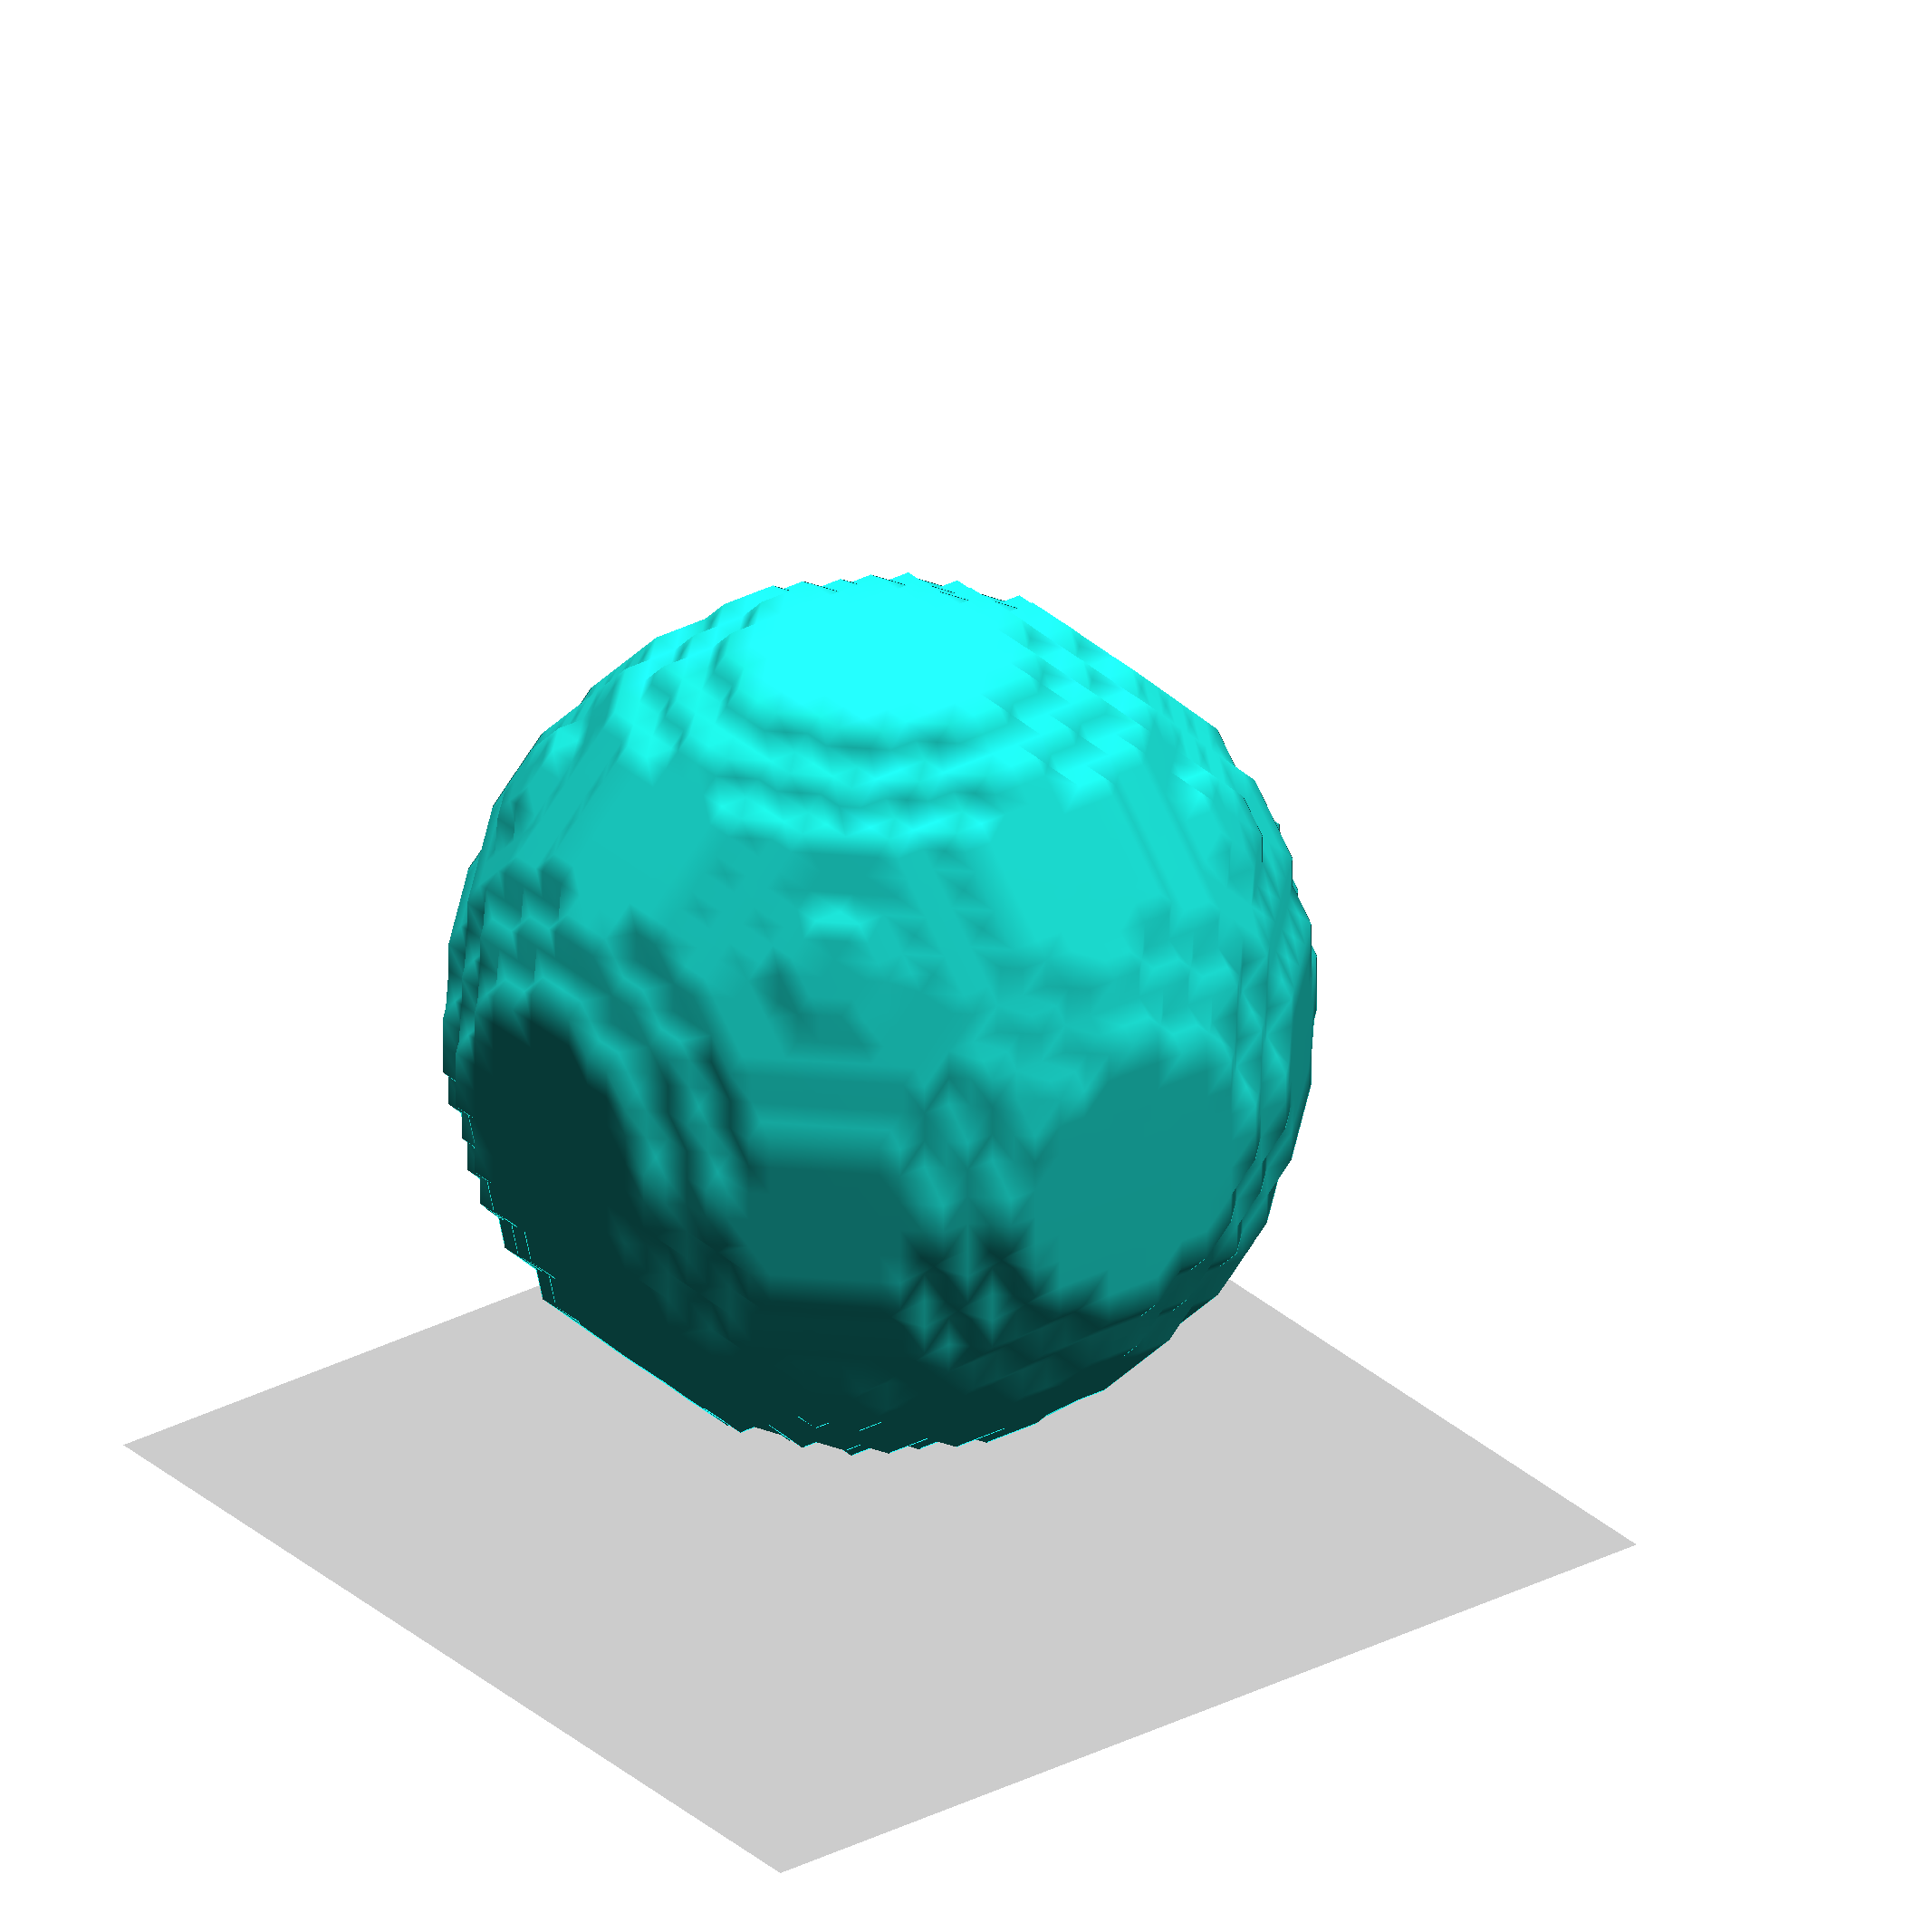
\includegraphics[width=0.18\linewidth]{chapter_background/img/binary_32x32x32.png} &
    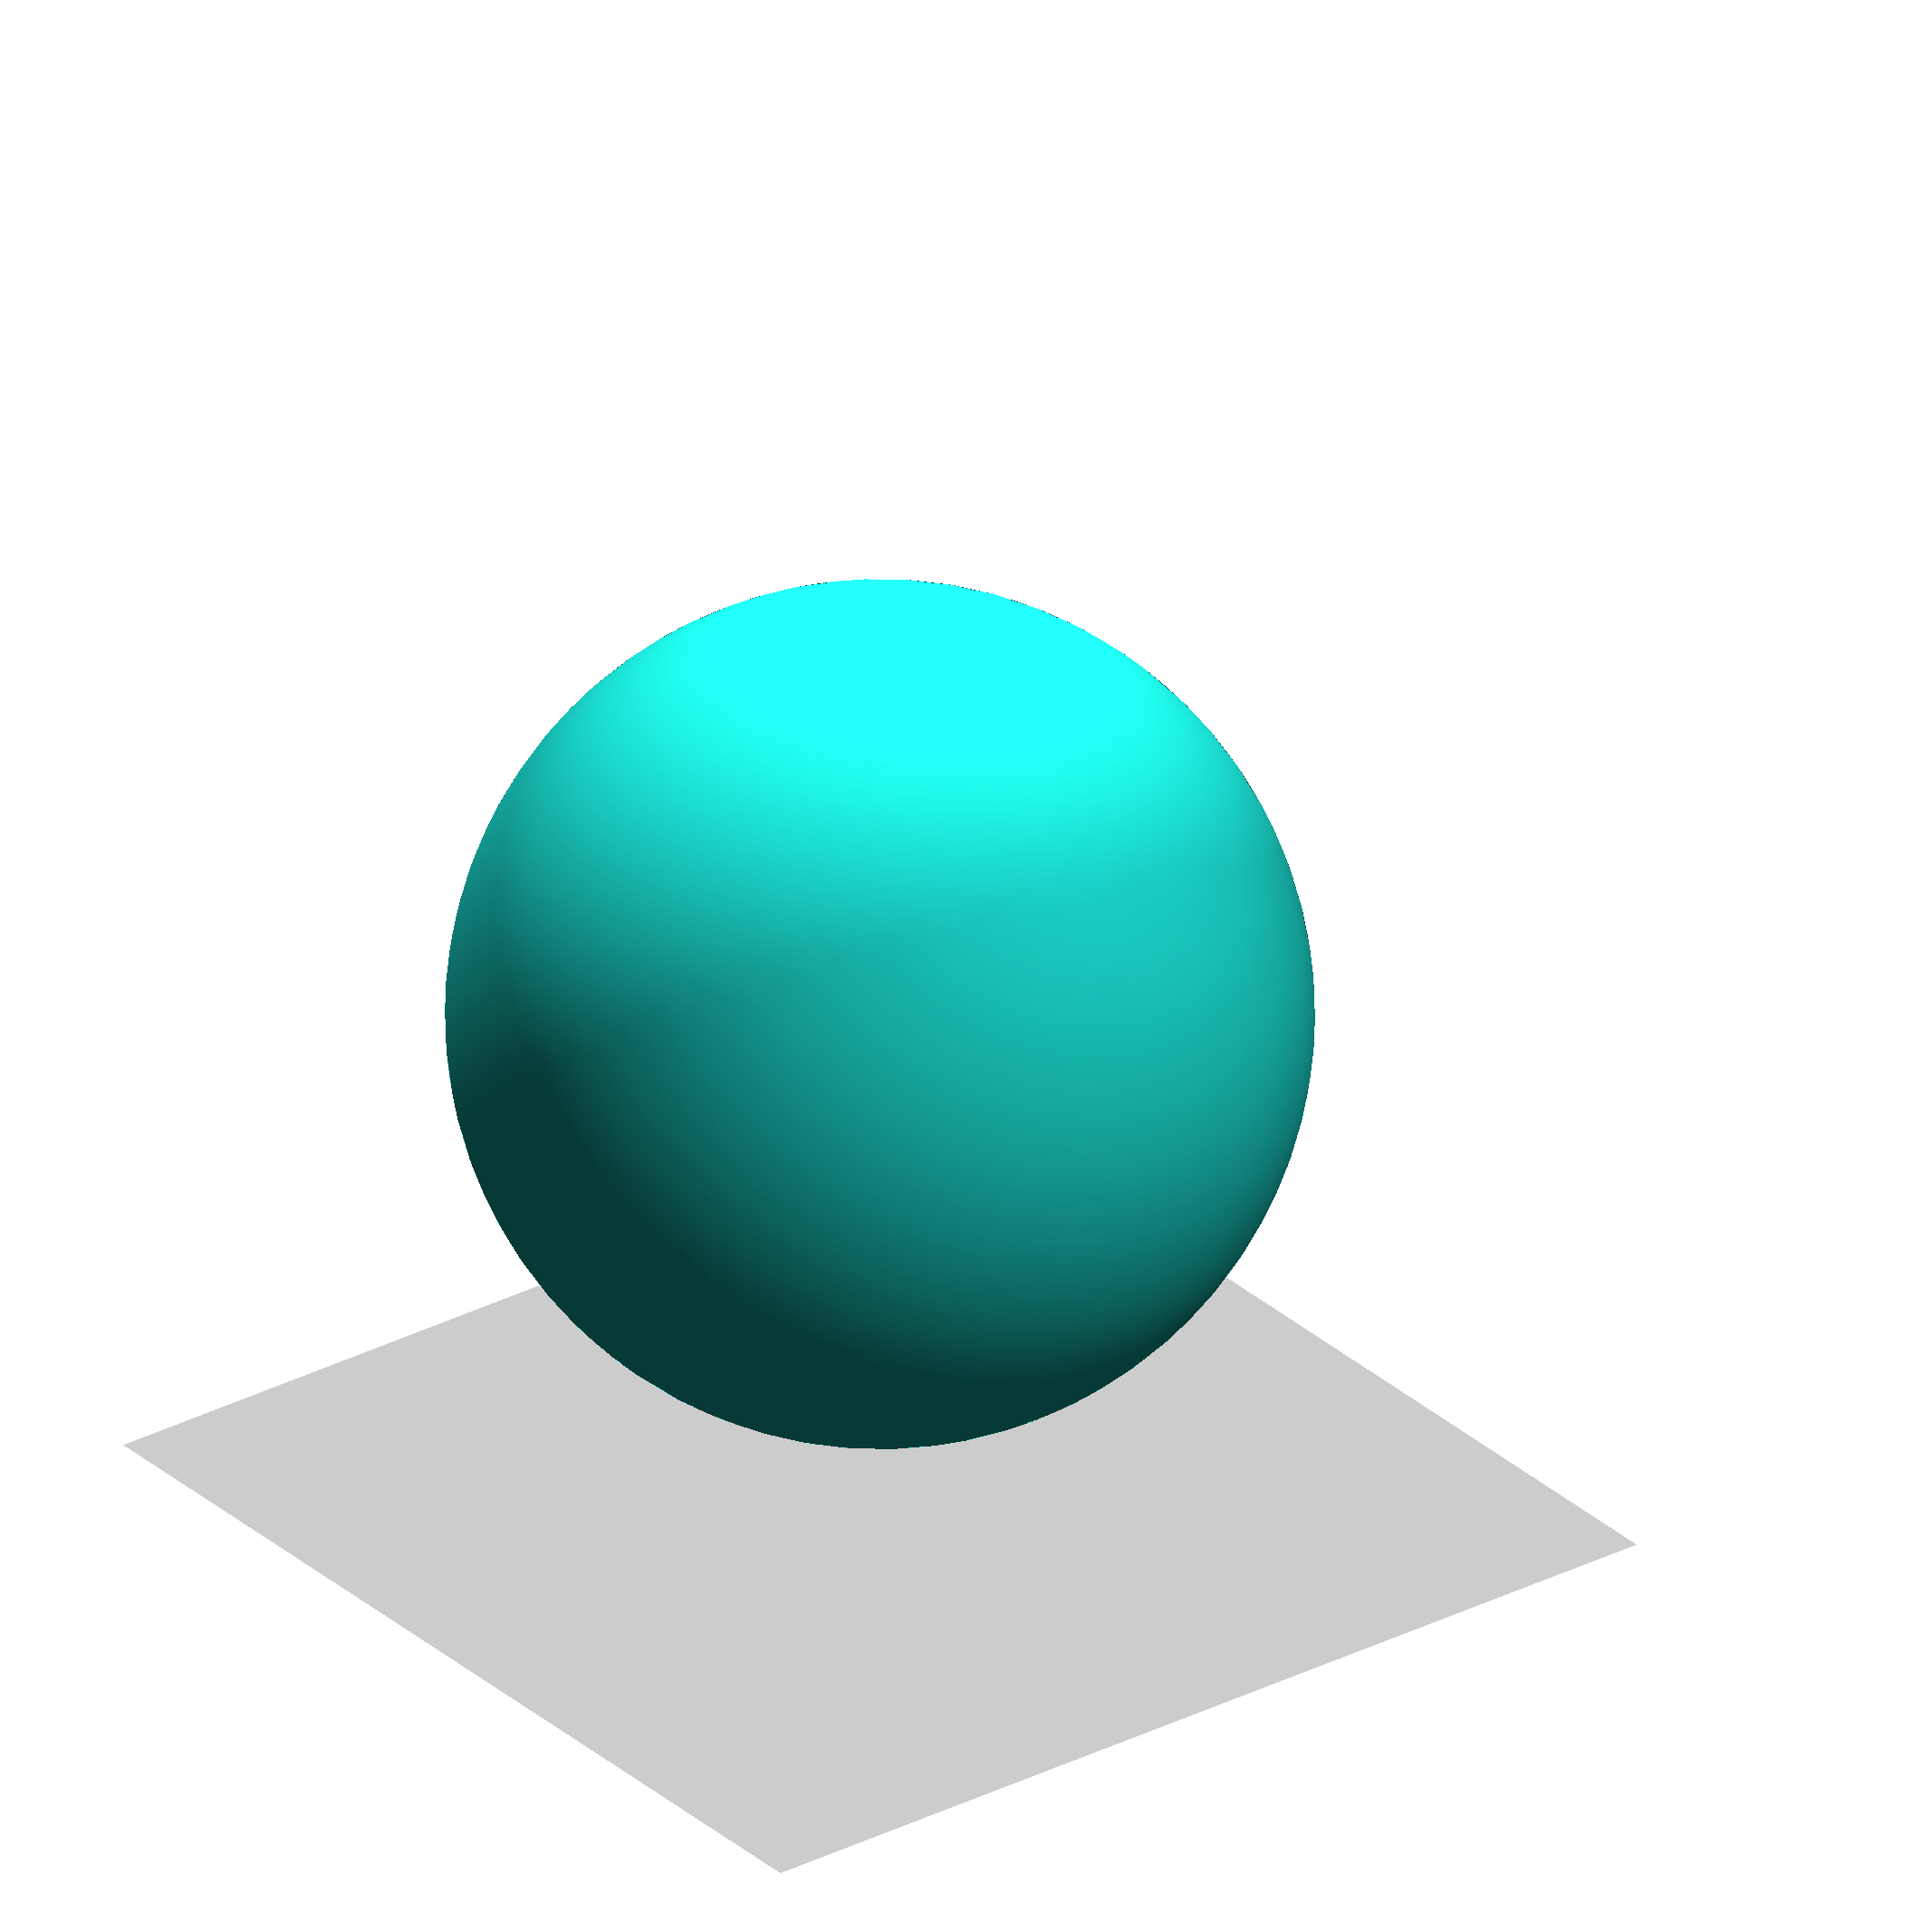
\includegraphics[width=0.18\linewidth]{chapter_background/img/real_32x32x32.png} &
    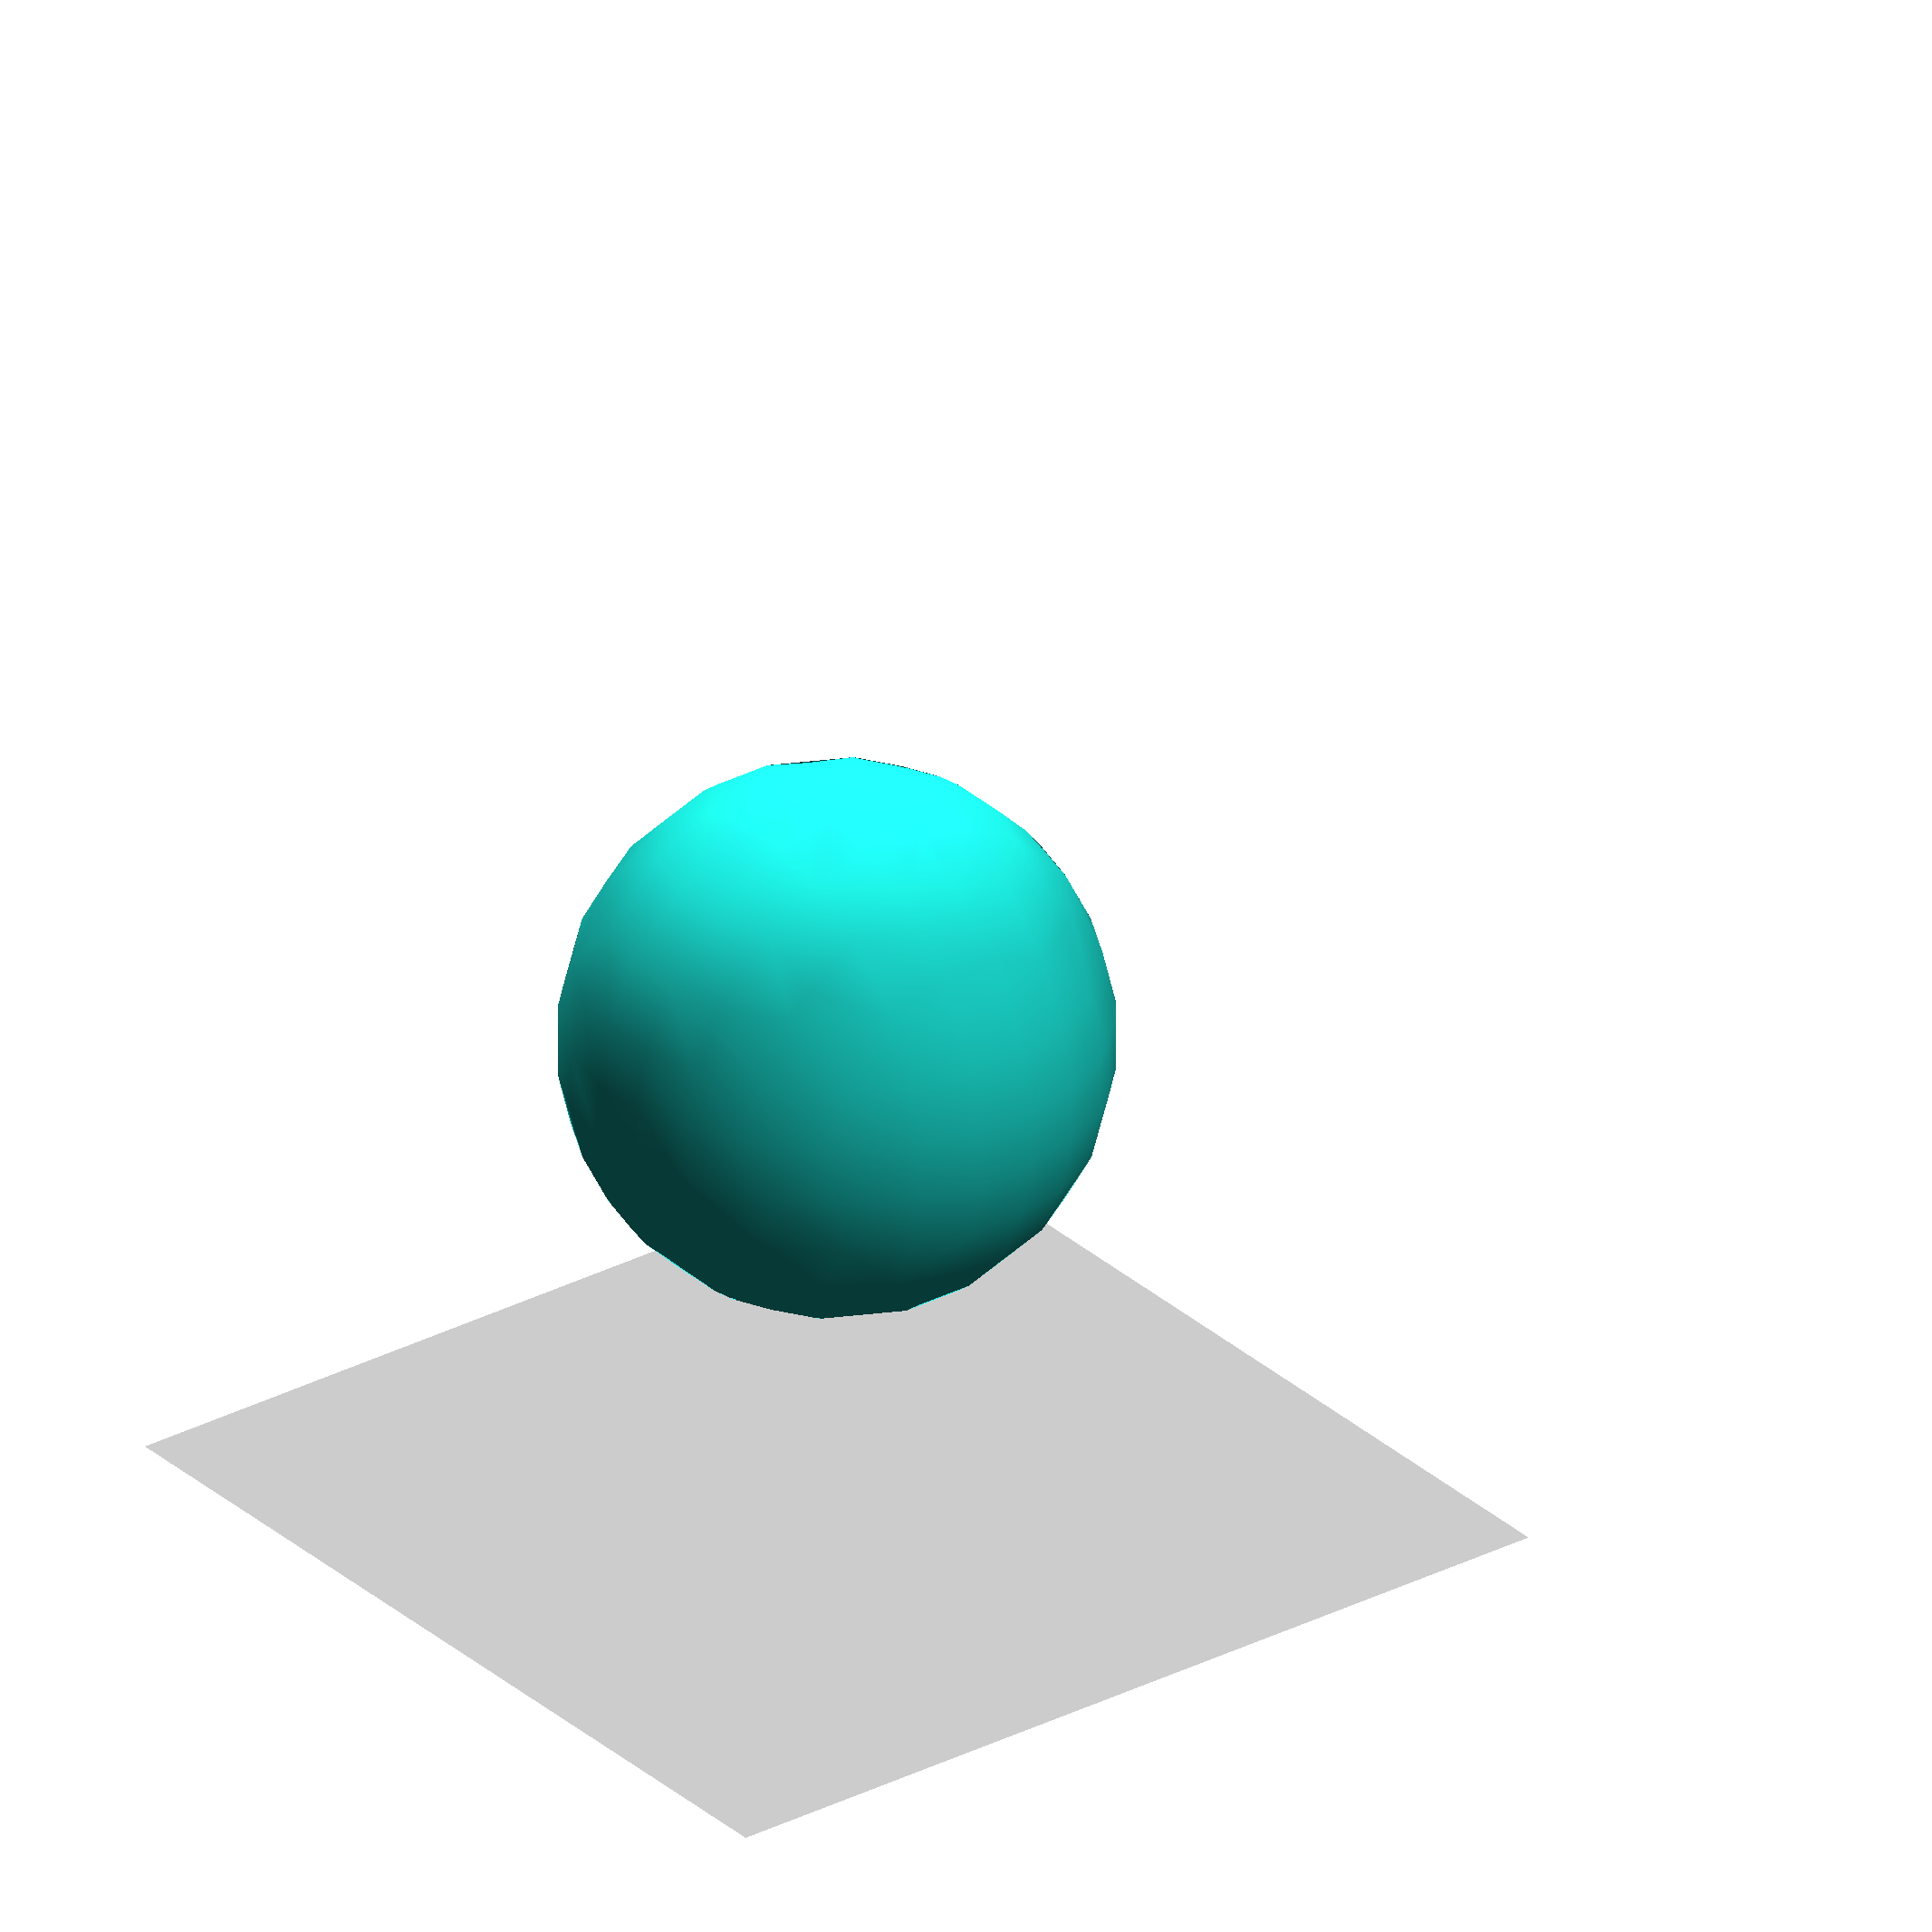
\includegraphics[width=0.18\linewidth]{chapter_background/img/real_16x16x16.png} &
    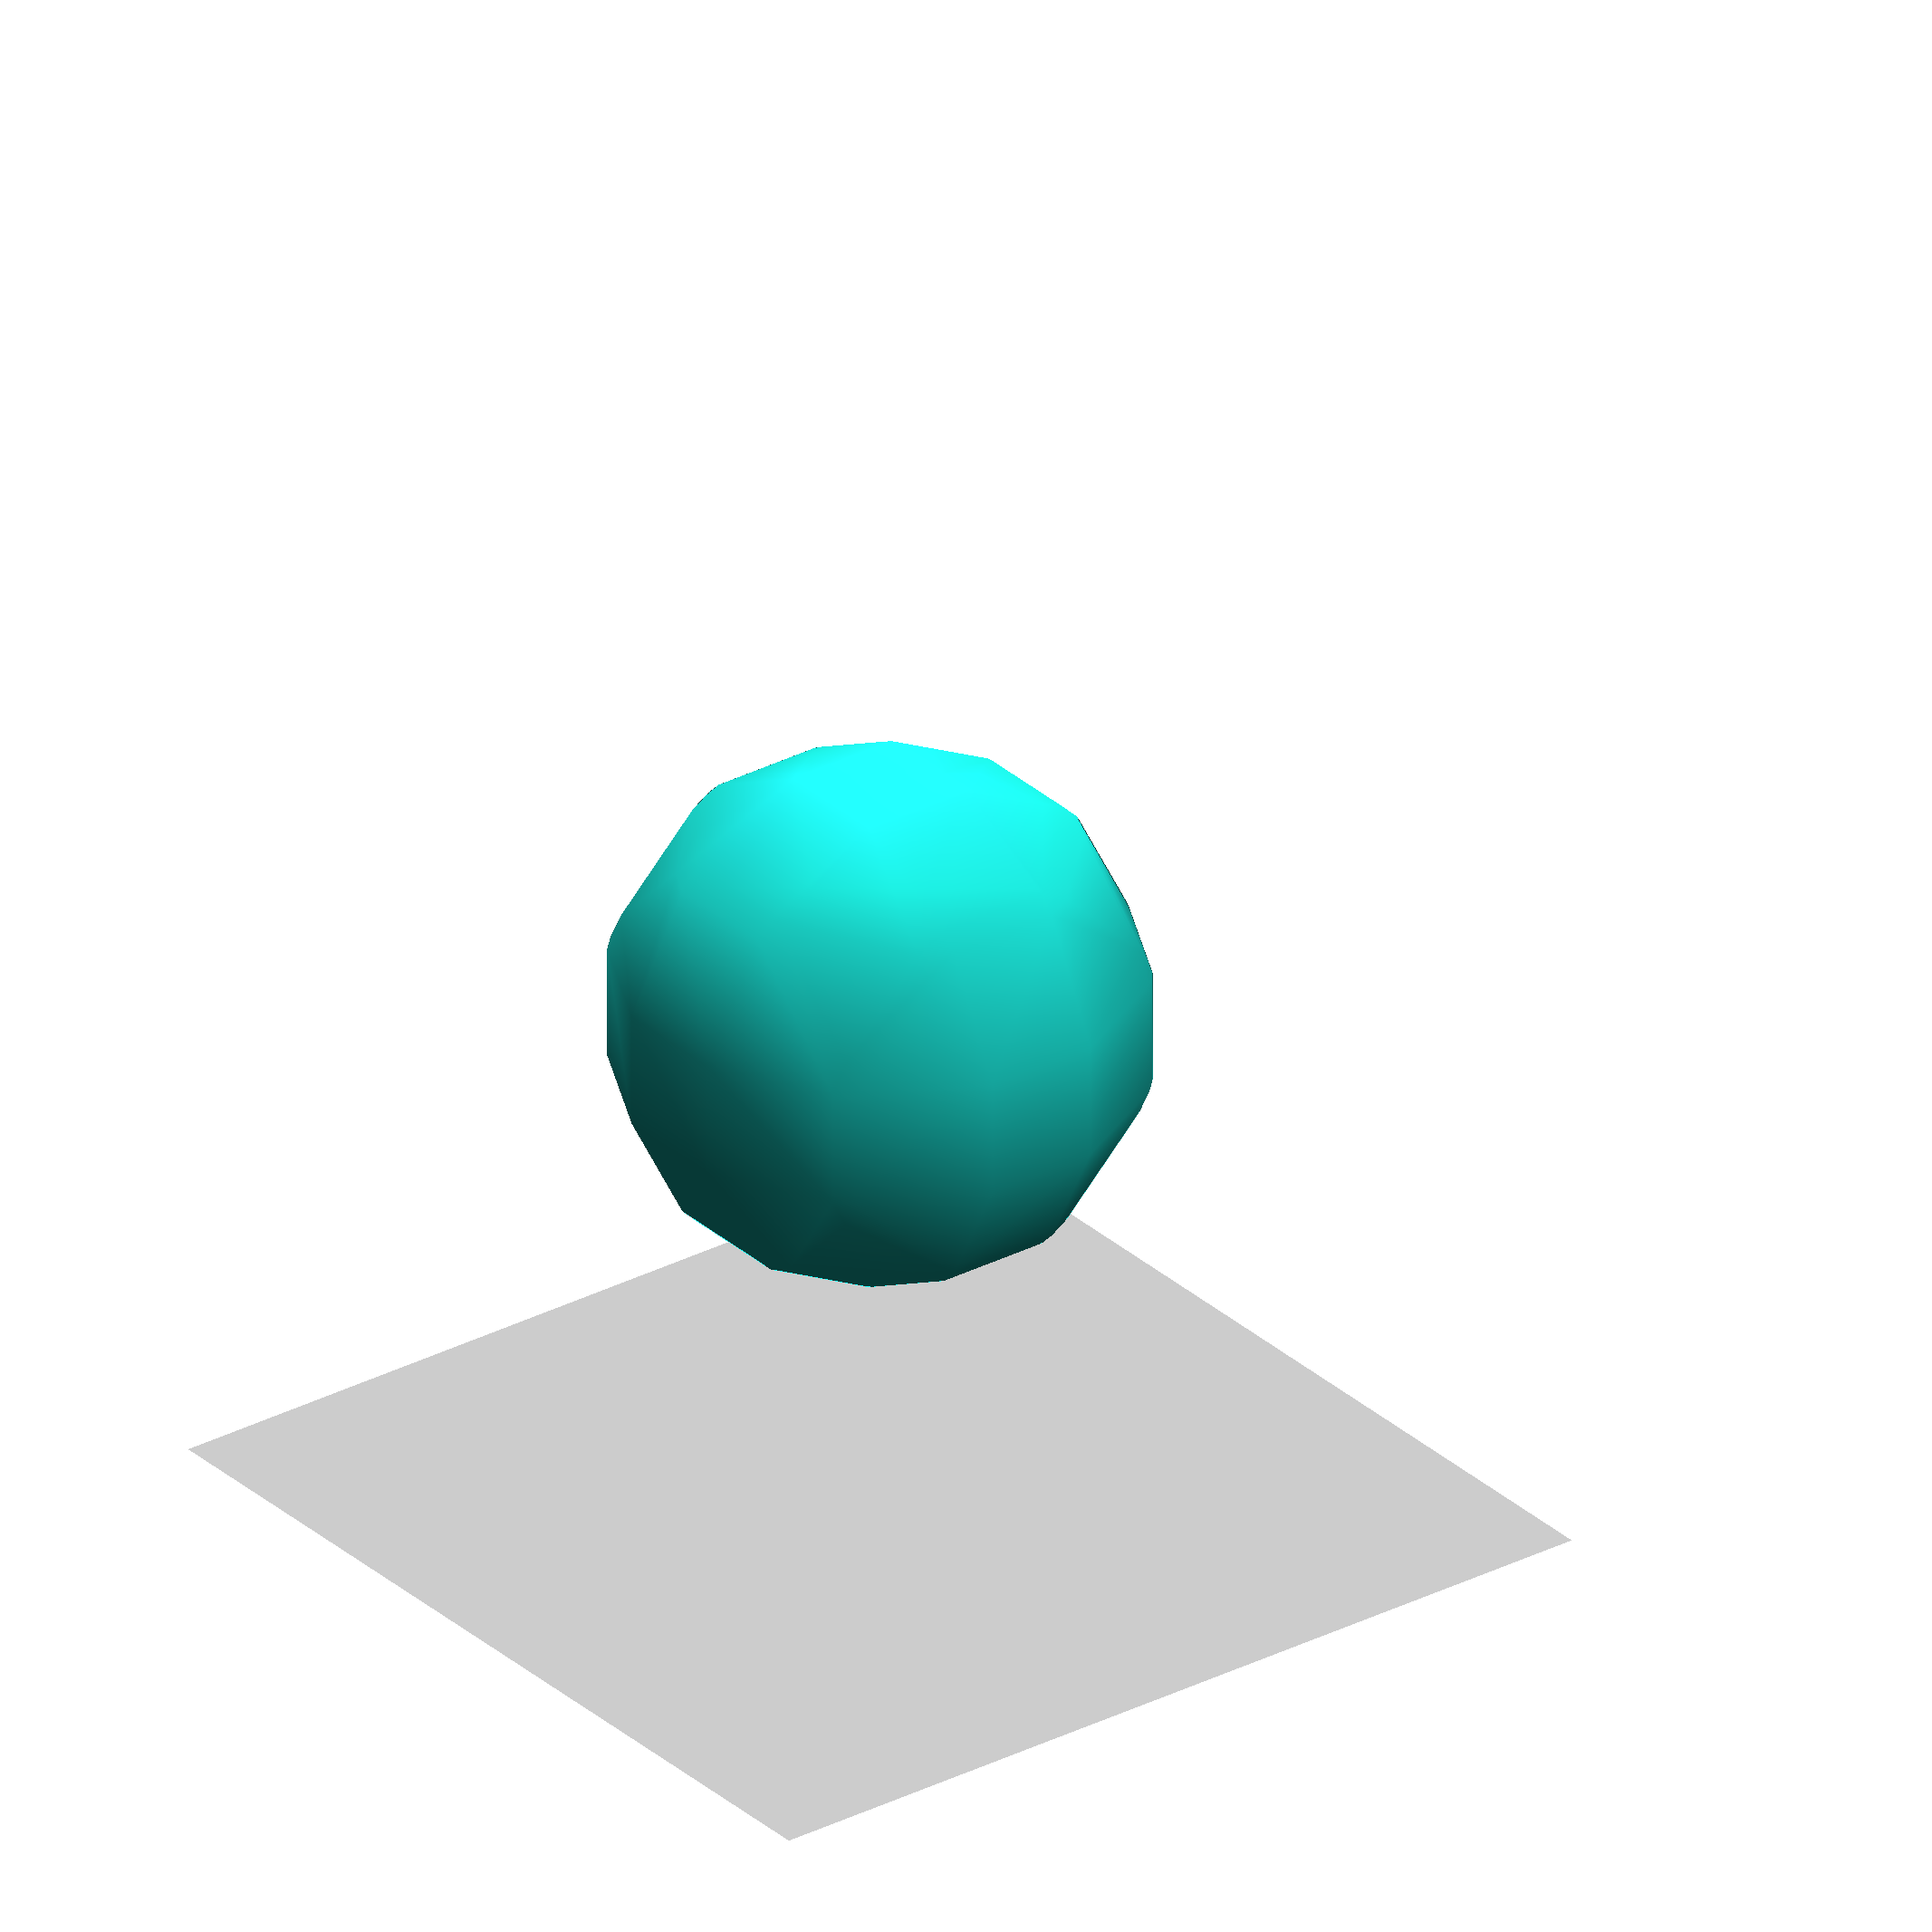
\includegraphics[width=0.18\linewidth]{chapter_background/img/real_8x8x8.png} &
    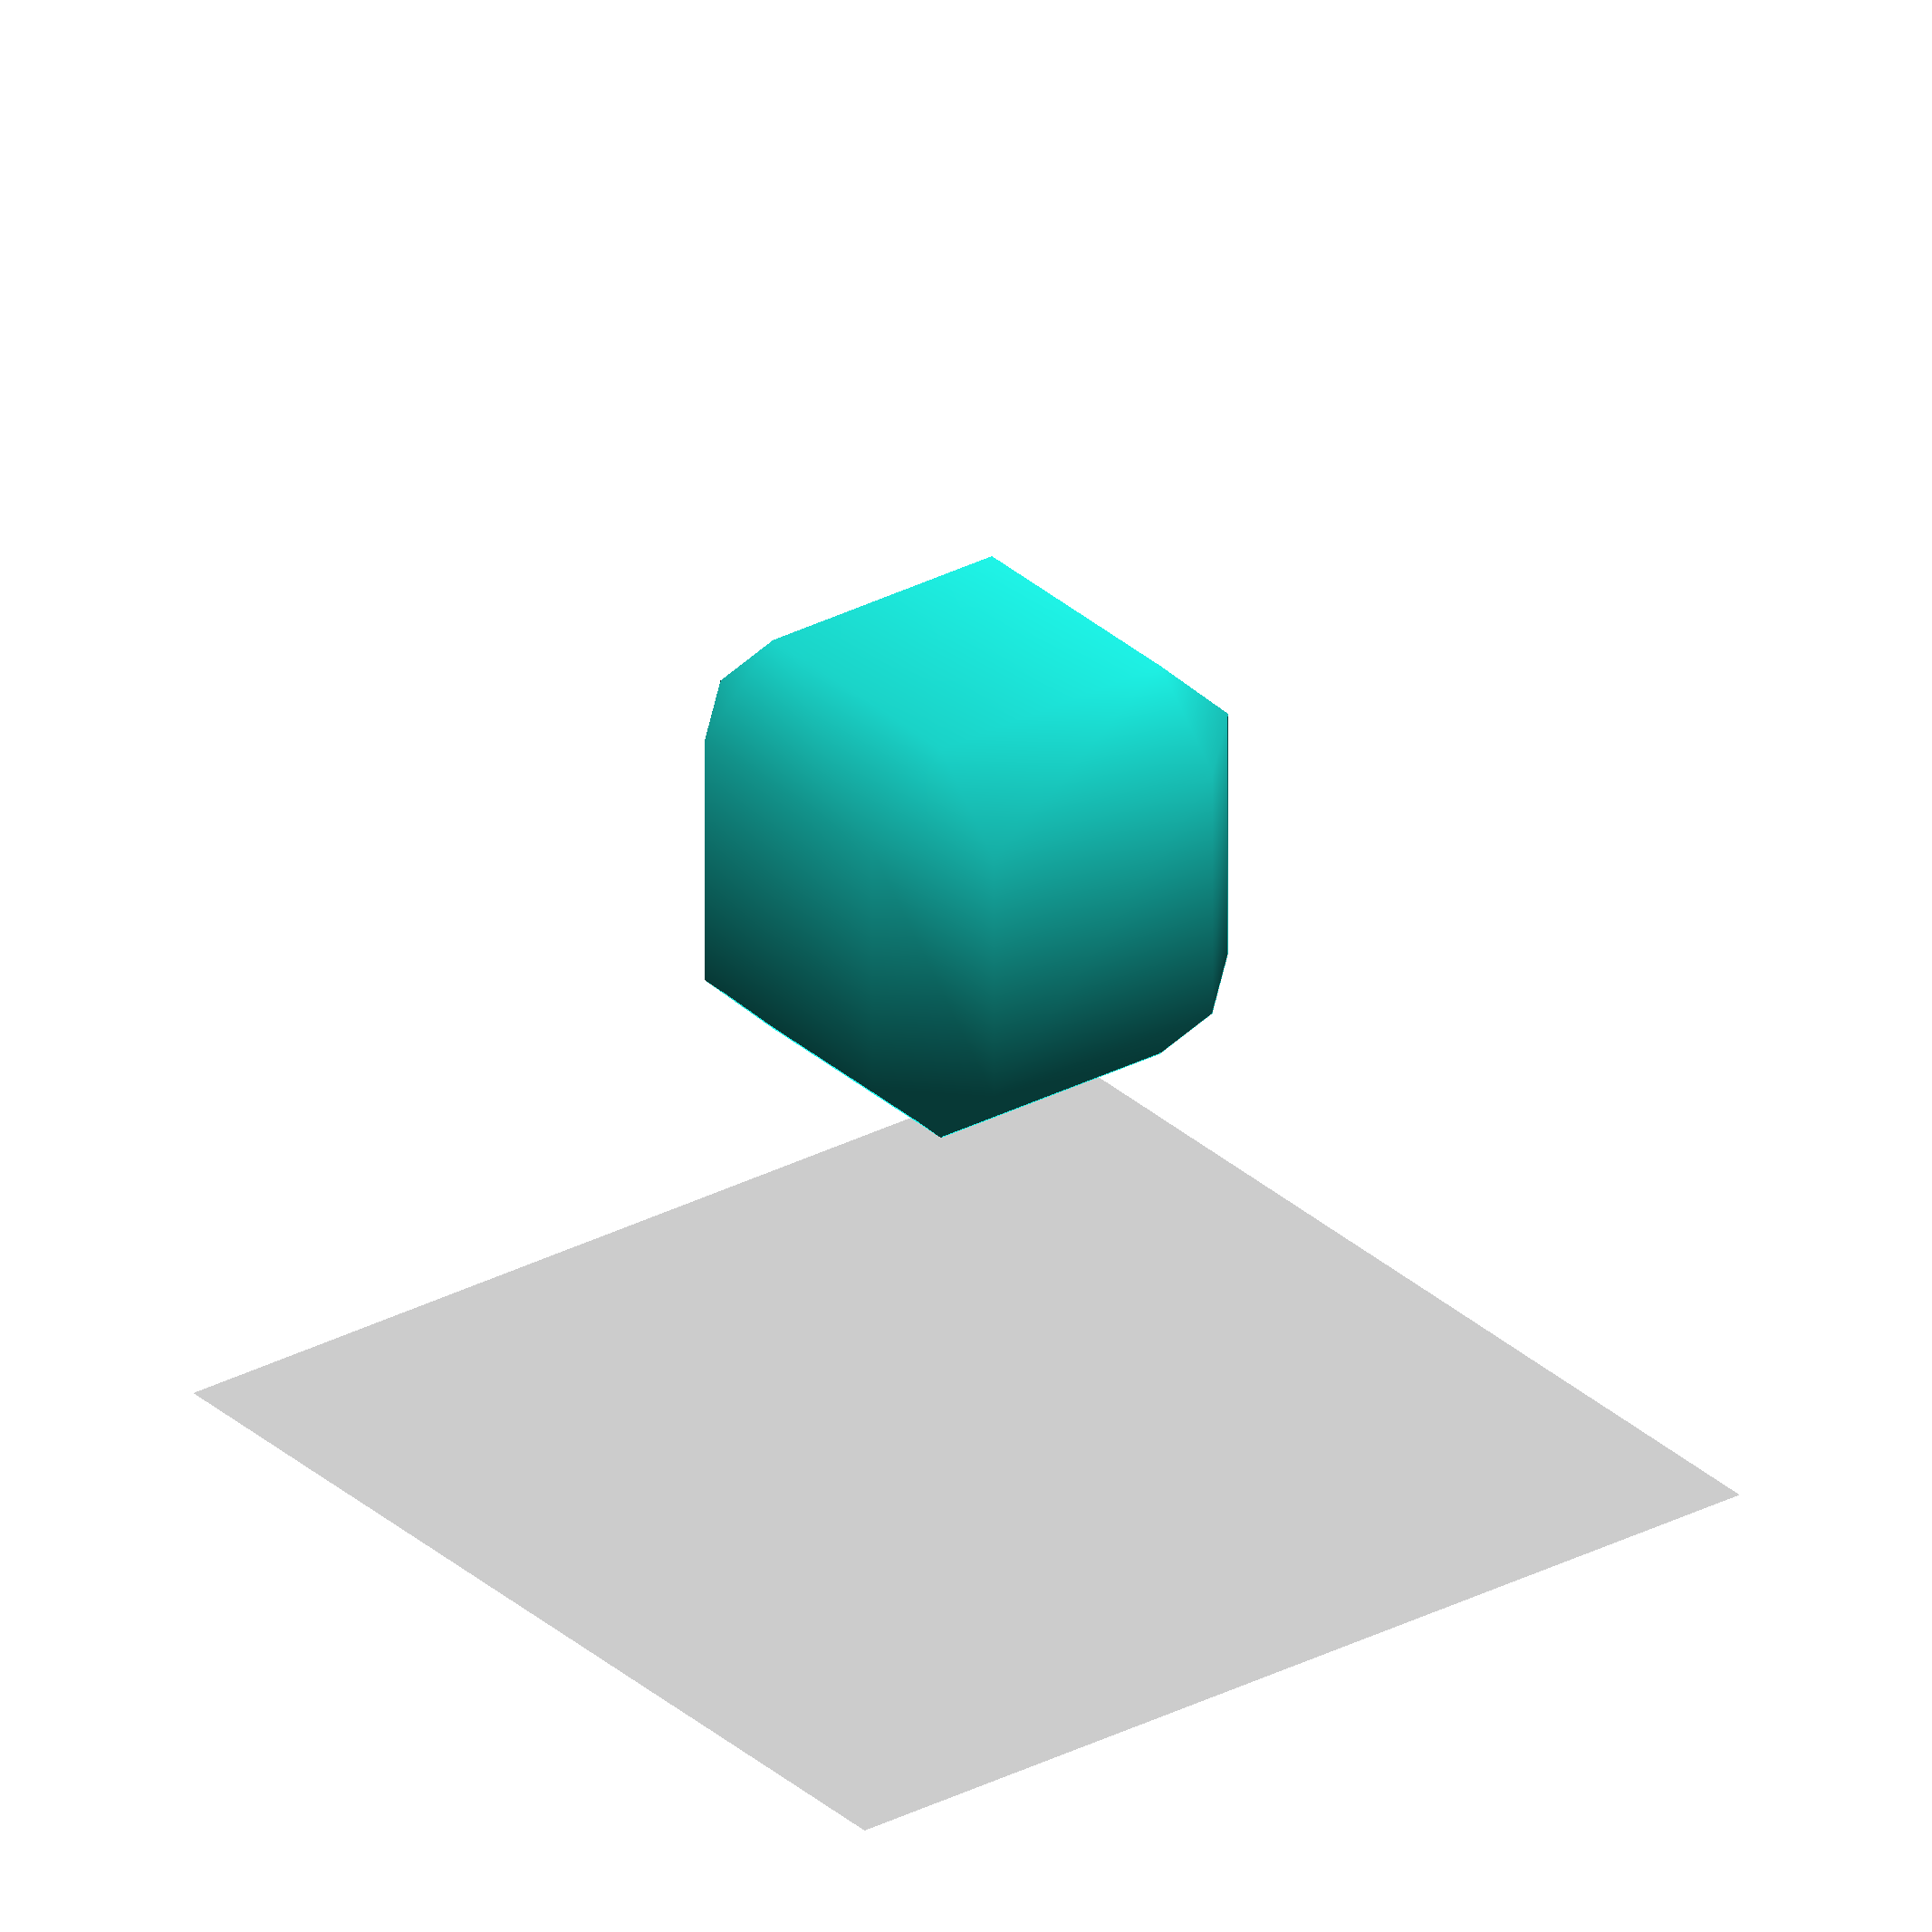
\includegraphics[width=0.18\linewidth]{chapter_background/img/real_4x4x4.png}
    \\
    Binary & Real & Real & Real & Real \\
    $32^3$ & $32^3$ & $16^3$ & $8^3$ & $4^3$ \\
  \end{tabular}
  \caption[Volumetric antialiasing at different resolutions]{A
    volumetric sphere, with and without antialiasing, at several
    different resolutions.}
  \label{fig:background:volquality}
\end{figure}

\subsection{Voxelisation}

The process of transforming a mesh into a volumetric structure is
referred to as voxelisation. Intuitively, this voxelisation process
discretises the mesh. It is no longer possible to reproduce a
non-integer form of the original mesh - a surface noticeably
constructed out of small cubes. Ideally, there should be minimal
visual degradation between viewing the original mesh and the voxelised
object.  Just as anti-aliasing is possible in 2D graphics, it is also
possible with 3D volumes. This is achieved by using real numbers
inside a voxel, instead of just a binary value.  This results in very
low distortion, provided the resolution is sensibly selected. This is
shown in Figure~\ref{fig:background:volquality}, the sphere encoded
using binary values is clearly built out of cubes, where as even a
small real value volume remains representative.

Generating a 2D image from 2D vector graphics (such as polygons) is
called rasterisation. This involves tracing a ray while counting the
number of line intersections. If the count is odd, colour in pixel and
move onto the next. If the count is even, just move onto the next
pixel. Voxelisation follows a similar idea, except it is performed in
three dimensions instead of two. This is done by tracing rays through
the X, Y and Z planes separately to produce three separate
volumes. These volumes are then combined in some way, typically by
ensuring each XYZ coordinate has been set in at least two volumes. We
show this visually in Figure~\ref{fig:background:voltracing}, where
error has been introduced by only voxelising the Stanford
Bunny\footnote{http://graphics.stanford.edu/data/3Dscanrep} from a
single direction.

\begin{figure}
  \centering
  \begin{tabular}{ccccc}
    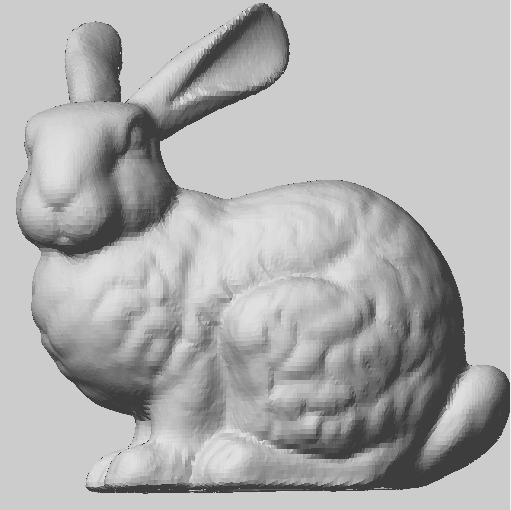
\includegraphics[width=0.17\linewidth]{imggen/vox_xyz/bunny_original.png} &
    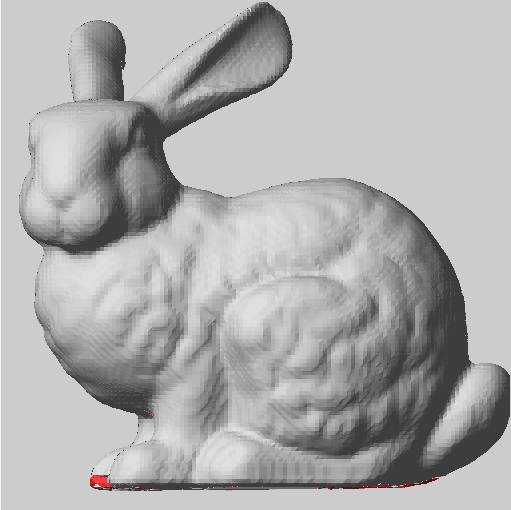
\includegraphics[width=0.17\linewidth]{imggen/vox_xyz/bunny_voxX.png} &
    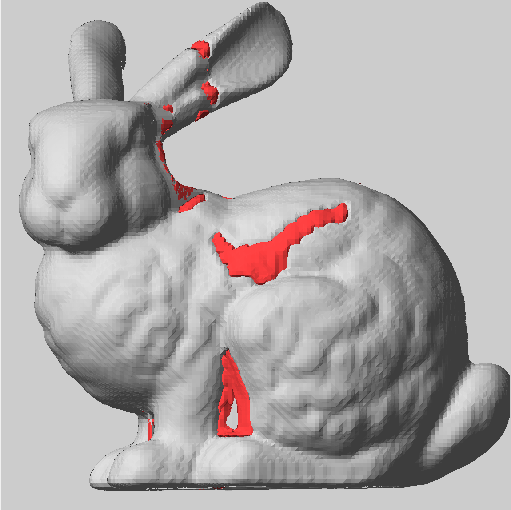
\includegraphics[width=0.17\linewidth]{imggen/vox_xyz/bunny_voxY.png} &
    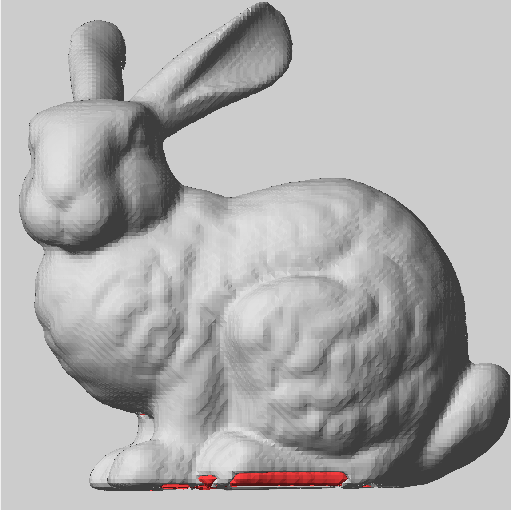
\includegraphics[width=0.17\linewidth]{imggen/vox_xyz/bunny_voxZ.png} &
    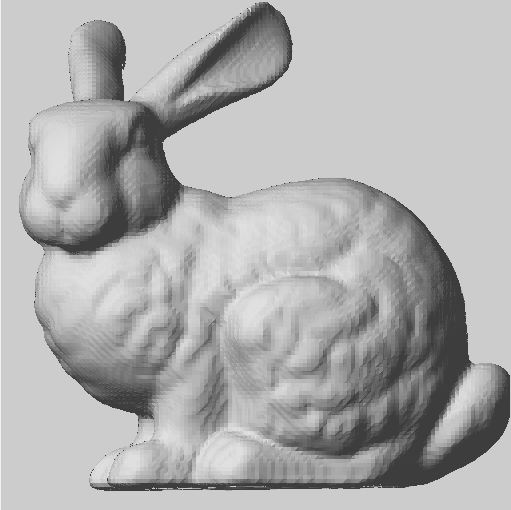
\includegraphics[width=0.17\linewidth]{imggen/vox_xyz/bunny_voxXYZ.png} \\
    Original & Voxelised & Voxelised & Voxelised & Voxelised \\
    Mesh     & Traced X  & Traced Y  & Traced Z  & Traced XYZ \\
  \end{tabular}
  \caption[Voxelisation error due to limiting ray tracing
  directions]{Voxelised results of the Stanford Bunny (original shown
    on left). The first three volumes have been voxelised by tracing
    from either X, Y or Z directions. The final volume (right most) is
    generated by voting. Red patches fill in voxels which have been
    missed. Each volume is $128^3$ in size.}
  \label{fig:background:voltracing}
\end{figure}

\subsection{Surface Extraction}

Surface extraction is the process of extracting a mesh which encloses
a 3D object represented in volumetric space. Occasionally such methods
require thresholds to extract separate regions of the volume, for
example, in an MRI scan, where the brain  needs to be visualised
independently of the skull (and hence, independently extracted from
the volume).

Perhaps the most popular method for computing the isosurface of a
volume is Marching Cubes~\cite{lorensen1987marching}, developed in
1987. The algorithm traverses through all voxels, using the value of
eight neighbouring voxels to form eight binary values, a single
byte. This byte can be used to lookup a known polygon configuration
from a table of $2^8 = 256$ entries. However, in the first version of
Marching Cubes, only 15 unique polygon configurations were
stored. This lead to cases of ambiguity when performing a lookup for
certain voxel configurations. The side effect of this is that meshes
would sometimes end up having holes in
them. In~\cite{chernyaev1995marching}, additional unique
configurations were proposed, leading to a total of 33. This removes
the ambiguity, and results in the meshes being closed or \textit{water
  tight}.


\subsection{Size, Compression and Formats}
\label{sec:background:volstorage}

There are many more factors which have to be considered when working
with volumetric representations of objects, as opposed to a standard
mesh.

To start with, the \textbf{size} of the volume (in terms of bytes)
grows much more rapidly than it would in a 2D image. In order to
represent a sensible amount of depth in a $128 \times 128$ image, a
volume of $128^3$ voxels is likely needed. If this is uncompressed and
encoded as bytes, it will require 2MB of storage. Scale this up to a
dataset of maybe 50,000 samples, use a slightly larger volume, and it
is clear that this may begin to cause problems.

One solution might be to compress the volumes. However, compression
introduces a significant computational overhead. It is a common trade
off between processing power, available storage and I/O speeds. While
compression of images has come a long way (even JPEG decoding is
hardware accelerated on some platforms now), the same is not true for
3D volumes. Generic file compression options are of course available
(Run Length Encoding, Huffman Coding and LZ77, just to name a few),
but on large volumes being read many times per second, the CPU could
easily become the bottleneck. In this work, we do not compress the
volumes and instead use large SSDs to store our volumetric training
data.

The format in which the volume is stored is another important
consideration. There are many formats for storing volumetric
data. Typically, these formats have been developed for the medical
field for use with MRI, CT scans and the like. As such, these formats
often include space for details such as patient information, along
with a metadata describing the resolution and bit depth of the
volumetric data. An argument can be made that none of this information
is required if the volumetric representation is used as an
intermediary state and doesn't have to be processed by
\textit{humans}. This applies to the work presented in this
thesis. The volumetric representation used in the work described
throughout this thesis is a contiguous array of bytes, which can be
very efficiently read into memory.


%%% Local Variables:
%%% TeX-master: "../thesis"
%%% End:
